% -*- latex -*-
%%%%%%%%%%%%%%%%%%%%%%%%%%%%%%%%%%%%%%%%%%%%%%%%%%%%%%%%%%%%%%%%
%%%%%%%%%%%%%%%%%%%%%%%%%%%%%%%%%%%%%%%%%%%%%%%%%%%%%%%%%%%%%%%%
%%%%
%%%% This text file is part of the source of 
%%%% `Parallel Programming in MPI and OpenMP'
%%%% by Victor Eijkhout, copyright 2012-2021
%%%%
%%%% mpi-moredata.tex : more about data
%%%%
%%%%%%%%%%%%%%%%%%%%%%%%%%%%%%%%%%%%%%%%%%%%%%%%%%%%%%%%%%%%%%%%
%%%%%%%%%%%%%%%%%%%%%%%%%%%%%%%%%%%%%%%%%%%%%%%%%%%%%%%%%%%%%%%%

\Level 0 {Type maps and type matching}

With derived types, you saw that it was not necessary for
the type of the sender and receiver to match.
Howver, when the send buffer is constructed,
and the receive buffer unpacked,
it is necessary for the successive types in that buffer to match.

The types in the send and receive buffers also need to match
the datatypes of the underlying architecture, with two exceptions.
The \indexmpishow{MPI_PACKED} and \indexmpishow{MPI_BYTE} types
can match any underlying type.
However, this still does not mean that it is a good idea to use
these types on only sender or receiver, and a specific type on the other.

\Level 0 {Type extent}
\label{sec:mpi-type-size}

See section~\ref{sec:mpi-type-match}
about the related issue of type sizes.

\Level 1 {Extent and true extent}

The \emph{datatype extent}\index{MPI!datatype!extent},
measured with
\indexmpiref{MPI_Type_get_extent},
is strictly the distance from the
first to the last data item of the type,
that is, with counting the gaps in the type.
It is measured in bytes so the output parameters are
of type \lstinline+MPI_Aint+.

\begin{figure}[ht]
  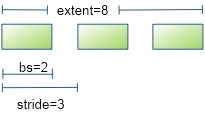
\includegraphics{extentvector}
  \caption{Extent of a vector datatype}
  \label{fig:extentvector}
\end{figure}

In the following example
(see also figure~\ref{fig:extentvector})
we measure the extent of a vector type.
Note that the extent is not the stride times the number of blocks,
because that would count a `trailing gap'.
%
\cverbatimsnippet[examples/mpi/c/typesize.c]{vectortypeextent}

Similarly, using \indexmpishow{MPI_Type_get_extent} counts the gaps
in a \lstinline{struct} induced by \indexterm{alignment} issues.
%
\cverbatimsnippet[examples/mpi/c/struct.c]{structextent}
%
See section~\ref{sec:data:struct} for the code defining the structure type.

\begin{remark}
  Routine \indexmpishow{MPI_Type_get_extent}
  replaces
  deprecated functions \indexmpidepr{MPI_Type_extent},
  \indexmpidepr{MPI_Type_lb}, \indexmpidepr{MPI_Type_ub}.
\end{remark}

The \emph{subarray datatype}\index{MPI!datatype!subarray} need not
start at the first element of the buffer, so the extent is an
overstatement of how much data is involved. The routine
\indexmpiref{MPI_Type_get_true_extent} returns the lower bound,
indicating where the data starts, and the extent from that point.

\begin{comment}
  Suppose we implement gather (see also Section Gather ) as a spanning
  tree implemented on top of point-to-point routines. Since the receive
  buffer is only valid on the root process, one will need to allocate
  some temporary space for receiving data on intermediate
  nodes. However, the datatype extent cannot be used as an estimate of
  the amount of space that needs to be allocated, if the user has
  modified the extent, for example by using MPI_TYPE_CREATE_RESIZED. The
  functions MPI_TYPE_GET_TRUE_EXTENT and MPI_TYPE_GET_TRUE_EXTENT_X are
  provided which return the true extent of the datatype.
\end{comment}

\cverbatimsnippet[examples/mpi/c/trueextent.c]{trueextent}

There is also a `big data' routine \indexmpishow{MPI_Type_get_true_extent_x}
that has an \indexmpishow{MPI_Count} as output.

\Level 1 {Extent resizing}

A type is partly characterized by its lower bound and extent,
or equivalently lower bound and upperbound.
Somewhat miraculously, you can actually change these to achieve special effects.
This is needed for some cases of gather/scatter operations, or when the count
of derived items in a buffer is more than one.

To understand the latter case, consider the vector type from the previous section.
It is clear that
\begin{lstlisting}
MPI_Type_vector( 2*count,bs,stride,oldtype,&two_n_type );
\end{lstlisting}
will not give the same result as
\begin{lstlisting}
MPI_Type_vector( count,bs,stride,oldtype,&one_n_type );
MPI_Type_contiguous( 2,&one_n_type,&two_n_type );
\end{lstlisting}

The problem here is that MPI uses the extent of the send type in a scatter,
or the receive type in a gather: if that type is 20 bytes big from
its first to its last element, then
data will be read out 20 bytes apart in a scatter, or written 20 bytes apart
in a gather. This ignores the `gaps' in the type!

The technicality on which the solution hinges is that you can `resize' a type
with \indexmpiref{MPI_Type_create_resized}
to give it a different extent, while not affecting how much data there
actually is in it.

\Level 2 {Example 1}

\begin{figure}[ht]
  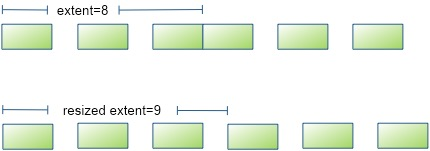
\includegraphics{extentpad}
  \caption{Effect of resizing a type}
  \label{fig:extentpad}
\end{figure}

First consider sending more than one derived type,
from a buffer containing consecutive integers:
%
\cverbatimsnippet[examples/mpi/c/vectorpadsend.c]{twovectorsend}
%
We receive into a contiguous buffer:
%
\cverbatimsnippet[examples/mpi/c/vectorpadsend.c]{twovectorrecv}
%
giving an output of:
\begin{verbatim}
Receive 6 elements: 0 2 4 5 7 9
\end{verbatim}
Next, we resize the type to ad the gap at the end.
This is illustrated in figure~\ref{fig:extentpad}.

Resizing the type looks like:
%
\cverbatimsnippet[examples/mpi/c/vectorpadsend.c]{twovectorpad}
%
and the corresponding output,
including querying the extents,
is:
\begin{verbatim}
Strided type l=0 e=20
Padded  type l=0 e=24
Receive 6 elements: 0 2 4 6 8 10
\end{verbatim}

\Level 2 {Example 2}

For another example, let's revisit exercise~\ref{ex:stridesend}
(and  figure~\ref{fig:stridesend})
where each process makes a
buffer of integers that will be interleaved in a gather call:
Strided data was sent in individual transactions.
Would it be possible to address all these interleaved packets in one
gather or scatter call?

\begin{lstlisting}
int *mydata = (int*) malloc( localsize*sizeof(int) );
for (int i=0; i<localsize; i++)
  mydata[i] = i*nprocs+procno;
MPI_Gather( mydata,localsize,MPI_INT,
    /* rest to be determined */ );
\end{lstlisting}

An ordinary gather call will of course not interleave, but
put the data end-to-end:
\begin{lstlisting}
MPI_Gather( mydata,localsize,MPI_INT,
            gathered,localsize,MPI_INT, // abutting
            root,comm );
\end{lstlisting}
\begin{verbatim}
gather 4 elements from 3 procs:
 0 3 6 9 1 4 7 10 2 5 8 11
\end{verbatim}

Using a strided type still puts data end-to-end, but now there
are unwritten gaps in the gather buffer:
\begin{lstlisting}
MPI_Gather( mydata,localsize,MPI_INT,
            gathered,1,stridetype, // abut with gaps
            root,comm );  
\end{lstlisting}
\begin{verbatim}
 0 1879048192 1100361260 3 3 0 6 0 0 9 1 198654
\end{verbatim}

\begin{figure}[ht]
  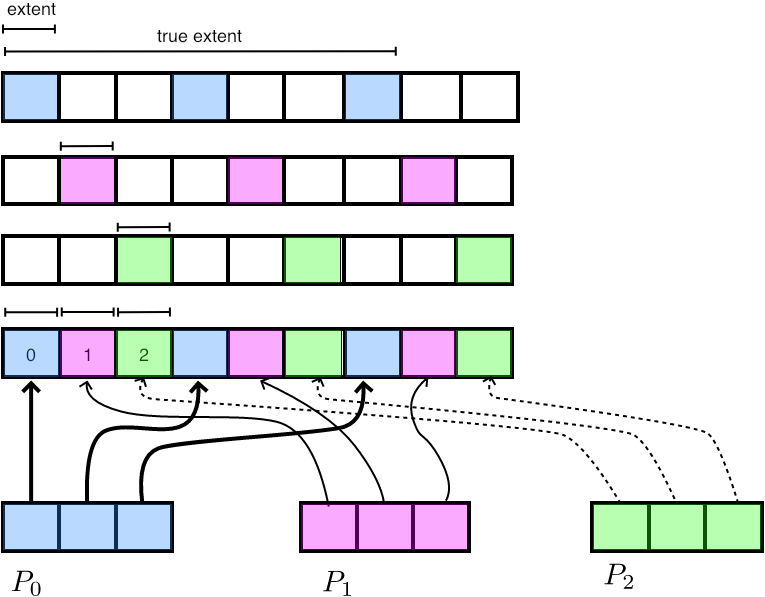
\includegraphics[scale=.4]{stride-extent}
  \caption{Interleaved gather from data with resized extent}
  \label{fig:stride-extent}
\end{figure}

The trick is to use \indexmpishow{MPI_Type_create_resized}
to make the extent of the type only one int long:
%
\cverbatimsnippet[examples/mpi/c/interleavegather]{interleavegather}
%
Now data is written with the same stride, but
at starting points equal to the shrunk extent:
\begin{verbatim}
 0 1 2 3 4 5 6 7 8 9 10 11
\end{verbatim}

This is illustrated in figure~\ref{fig:stride-extent}.

\begin{exercise}[stridesend]
  \label{ex:stridesendsized}
  Rewrite exercise~\ref{ex:stridesend} to use a gather,
  rather than individual messages.
\end{exercise}

\begin{mplnote}{Extent resizing}
  Resizing a datatype does not give a new type, but
  does the resize `in place':
\begin{lstlisting}
void layout::resize(ssize_t lb, ssize_t extent);
\end{lstlisting}
\end{mplnote}

\Level 2 {Example: dynamic vectors}

Does it bother you (a little) that in the vector type you
have to specify explicitly how many blocks there are?
It would be nice if you could create a `block with padding'
and then send however many of those.

Well, you can introduce that padding by resizing a type,
making it a little larger.

\cverbatimsnippet[examples/mpi/c/stridestretch.c]{paddedblock1}

There is a second solution to this problem, using a structure type.
This does not use resizing, but rather indicates a displacement
that reaches to the end of the structure. We do this
by putting a type \indexmpishow{MPI_UB} at this displacement:

\cverbatimsnippet[examples/mpi/c/stridestretch.c]{paddedblock2}

\Level 2 {Example: transpose}
\index{transpose!through derived types|(}

\begin{figure}[ht]
  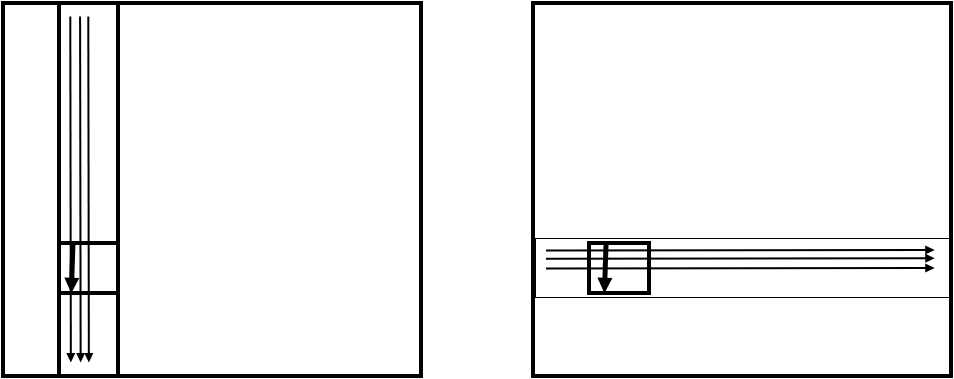
\includegraphics[scale=.3]{transposetype}
  \caption{Transposing a 1D partitioned array}
  \label{fig:transposetype} 
\end{figure}
Transposing data is an important part of such operations as the \ac{FFT}.
We develop this in steps. Refer to figure~\ref{fig:transposetype}.

The source data can be described as a vector type defined as:
\begin{itemize}
\item there are $b$ blocks,
\item of blocksize $b$,
\item spaced apart by the global $i$-size of the array.
\end{itemize}
% this is an exercise, so no source listed
\cverbatimsnippet{transposesrctype} % in an exerccise

The target type is harder to describe.
First we note that each contiguous block from the source type
can be described as a vector type with:
\begin{itemize}
\item $b$ blocks,
\item of size~1 each,
\item stided by the global $j$-size of the matrix.
\end{itemize}
%
\cverbatimsnippet{transposetarlinetype}% in an exercise

For the full type at the receiving process we now need to pack
$b$ of these lines together.

\begin{exercise}
  Finish the code.
  \begin{itemize}
  \item
    What is the extent of the \lstinline{targetcolumn} type?
  \item What is the spacing of the first elements of the blocks? How
    do you therefore resize the \lstinline{targetcolumn} type?
  \end{itemize}
\end{exercise}

\index{transpose!through derived types|)}

\Level 0 {Reconstructing types}

It is possible to find from a datatype how it was constructed.
This uses the routines
\indexmpidef{MPI_Type_get_envelope} and
\indexmpidef{MPI_Type_get_contents}.
The first routine returns the \indexterm{combiner}
(with values such as \indexmpidef{MPI_COMBINER_VECTOR})
and the number of parameters;
the second routine is then used to retrieve the actual parameters.

\begin{comment}
  \Level 1 {Datatype signatures}
  \label{sec:signature}
  \index{datatype!signature|(}

  With the primitive types it pretty much went
  without saying that if the sender sends an array of doubles, the
  receiver had to declare the datatype also as doubles. With derived
  types that is no longer the case: the sender and receiver can declare
  a different datatype for the send and receive buffer, as long as these
  have the same \indextermbus{datatype}{signature}.

  The signature of a datatype is the internal representation of that
  datatype. For instance, if the sender declares a datatype consisting
  of two doubles, and it sends four elements of that type, the receiver
  can receive it as two elements of a type consisting of four doubles.

  You can also look at the signature as the form `under the hood' in which MPI
  sends the data.

  \index{datatype!signature|)}
\end{comment}

\Level 0 {Packing}
\label{sec:pack}

One of the reasons for derived datatypes is dealing with noncontiguous data.
In older communication libraries this could only be done by \indexterm{packing} data
from its original containers into a buffer, and likewise unpacking it at the
receiver into its destination data structures.

MPI offers this packing facility, partly for compatibility with such libraries,
but also for reasons of flexibility. Unlike with derived datatypes,
which transfers data atomically, packing routines add data sequentially
to the buffer and unpacking takes them sequentially. 

This means that 
one could pack an integer describing how many floating point numbers
are in the rest of the packed message. 
Correspondingly, the unpack routine could then investigate the first integer
and based on it unpack the right number of floating point numbers.

MPI offers the following:
\begin{itemize}
\item The \indexmpishow{MPI_Pack} command adds data to a send buffer;
\item the \indexmpishow{MPI_Unpack} command retrieves data from a receive buffer;
\item the buffer is sent with a datatype of \indexmpishow{MPI_PACKED}.
\end{itemize}

With \indexmpishow{MPI_Pack} data elements can be added 
to a buffer one at a time. The \n{position} parameter is updated
each time by the packing routine.
\begin{lstlisting}
int MPI_Pack(
  void *inbuf, int incount, MPI_Datatype datatype,
  void *outbuf, int outcount, int *position,
  MPI_Comm comm);
\end{lstlisting}

Conversely, \indexmpishow{MPI_Unpack} retrieves one element
from the buffer at a time. You need to specify the MPI datatype.
\begin{lstlisting}
int MPI_Unpack(
  void *inbuf, int insize, int *position,
  void *outbuf, int outcount, MPI_Datatype datatype,
  MPI_Comm comm);
\end{lstlisting}

A packed buffer is sent or received with a datatype of
\indexmpishow{MPI_PACKED}. The sending routine uses the \n{position}
parameter to specify how much data is sent, but the receiving routine
does not know this value a~priori, so has to specify an upper bound.

\cverbatimsnippet[examples/mpi/pack/pack.c]{packunpack}

You can precompute the size of the required buffer with
%
\indexmpiref{MPI_Pack_size}
%
Add one time \indexmpishow{MPI_BSEND_OVERHEAD}.

\begin{exercise}
  \label{ex:packAOS}
  Suppose you have a `structure of arrays'
\begin{lstlisting}
struct aos {
  int length;
  double *reals;
  double *imags;
};
\end{lstlisting}
  with dynamically created arrays. Write code to send and receive this
  structure.
\end{exercise}
